\section{Simulation Architecture and Shared Conventions}
\label{sec:architecture}

\subsection{Physical truth, measurements, and estimates}
The physical branch computes loads and mass properties and integrates vehicle motion. The measurement branch samples that truth through sensor error and availability models. Navigation propagates its own attitude and estimates the IMU-station motion. Comparison uses the same station and time. Figure~\ref{fig:architecture} separates these interfaces.

\par\medskip\noindent\begin{minipage}{\linewidth}
\centering
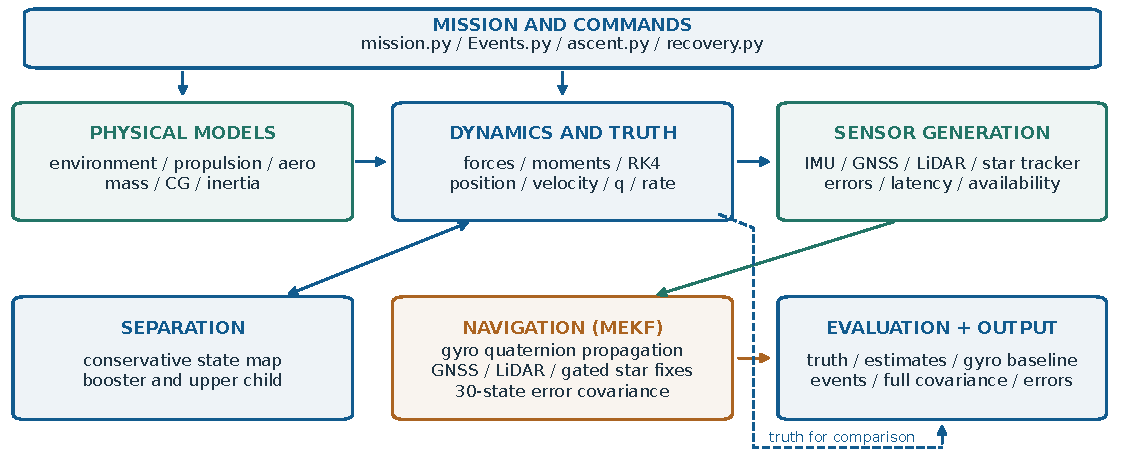
\includegraphics[width=0.97\linewidth]{images/simulation_architecture.pdf}
\captionof{figure}{Implemented data flow. The MEKF uses simulated sensor measurements and its own propagated attitude. Truth supplies sensor generation and evaluation; initial alignment is assumed. Return commands use physical-state feedback, while navigation is evaluated separately.}
\label{fig:architecture}
\end{minipage}\par\medskip

The mission layer selects the initial configuration, commands, and accepted phase. A throttle command becomes thrust and flow through propulsion; an aerodynamic configuration and fin command become force and moment through aerodynamics. The dynamics model then calculates the resulting motion. Neither the force provider nor the mass model prescribes the reference altitude/speed history. Table~\ref{tab:architecture-modules} assigns the corresponding implementation responsibilities.

\par\medskip\noindent\begin{minipage}{\linewidth}
\centering\small
\begin{tabularx}{\linewidth}{@{}p{0.22\linewidth}p{0.35\linewidth}X@{}}
\toprule
Function & Main modules & Interface \\
\midrule
Vehicle properties & \path{VehicleData.py}\newline\path{vehicle_mass_model.py}\newline\path{mass_properties.py} & Trial inventory to mass, CG, inertia, and derivatives. \\
Environment and loads & \path{Environement.py}\newline\path{propulsion.py}\newline\path{Aerodynamics.py}\newline\path{load_interface.py} & Trial state/commands to loads and exhaust data. \\
Motion and configuration & \path{dynamics.py}\newline\path{frames.py}\newline\path{staging.py} & Derivative, integrated state, and inherited child states. \\
Measurement and estimation & \path{sensors.py}\newline\path{kalman.py} & Sensor-station truth to observations and separate estimates. \\
Mission execution & \path{main.py}\newline\path{mission.py}\newline\path{Events.py} & Commands, accepted clocks/events, state synchronization, and saved output. \\
\bottomrule
\end{tabularx}
\captionof{table}{Responsibilities of the shared implementation. Configuration and scenario decisions are kept separate from reusable component arithmetic and equations of motion.}
\label{tab:architecture-modules}
\end{minipage}\par\medskip

\subsection{Frames, origins, and attitude convention}
Frame $B$ is right-handed and fixed to the vehicle, with $+x_B$ toward the nose. Frame $E$ is Earth-centred, launch-aligned, and rotating with Earth. Code identifiers call it ECEF, but its axes are not conventional Greenwich-axis ECEF. At the launch site, $+x_E$ is north, $-y_E$ east, and $+z_E$ up; the initial structural base is $[0,0,R_E]^{\mathsf T}$ with $R_E=6371000\,\mathrm{m}$.

The scalar-first Hamilton quaternion $\vect q_{BE}=[q_w,q_x,q_y,q_z]^{\mathsf T}$ maps Body components into $E$ using $\mat C_{BE}$. Equation~\eqref{eq:frame-initialization} defines the vector transformation and launch orientation:
\begin{equation}
 \vect u^E=\mat C_{BE}\vect u^B,\qquad
 \vect q_{BE}(0)=\begin{bmatrix}\sqrt{1/2}&0&-\sqrt{1/2}&0\end{bmatrix}^{\mathsf T},
 \qquad
 \mat C_{BE}(0)=\begin{bmatrix}0&0&-1\\0&1&0\\1&0&0\end{bmatrix}.
\label{eq:frame-initialization}
\end{equation}
Thus Body $+x$ is initially upward, Body $+y$ maps to $+y_E$, and Body $+z$ maps to $-x_E$. Quaternions are normalized, and $\vect q$ and $-\vect q$ denote the same orientation. The adopted latitude $\lambda=28.6^\circ$ rotates the Earth-rate vector into the launch-aligned frame as $\vect\Omega^E=\Omega_E[\cos\lambda,0,\sin\lambda]^{\mathsf T}$, with $\Omega_E=7.292115\times10^{-5}\,\mathrm{rad\,s^{-1}}$. It does not relocate the pad into Greenwich-axis coordinates.

Reference point and component basis are separate choices. Table~\ref{tab:state-origins} distinguishes them. A structural station $\vect s^B$ is measured from the stage base, whereas the corresponding CG force arm is $\vect d^B=\vect s^B-\vect c^B$, where $\vect c^B$ is the current CG station.

\begin{table}[!htbp]
\centering\small
\begin{tabularx}{\linewidth}{@{}p{0.31\linewidth}X@{}}
\toprule
Quantity & Meaning \\
\midrule
Dynamic position $\vect r_C^B$ & Earth centre to instantaneous CG, expressed in current Body axes. \\
Dynamic velocity $\vect v_C^B$ & CG velocity relative to rotating Earth, in current Body components. \\
Vehicle-object position/velocity & Structural-base state, with the same external origin and Body component basis. \\
Component/sensor station $\vect s^B$ & Fixed structural location measured from the relevant stage base. \\
Moment and inertia & About the instantaneous vehicle CG, in Body axes. \\
Filter position/velocity & At the fixed IMU station, expressed in frame $E$. \\
\bottomrule
\end{tabularx}
\caption{Shared origins and representations. Storing an Earth-centred vector in Body components does not make its origin the CG.}
\label{tab:state-origins}
\end{table}

\subsection{Physical and estimated states}
The physical state contains 15 stored numbers: three CG-position components, three CG-velocity components, four quaternion components, three angular-rate components, and two stage-indexed propellant inventories. The unit-quaternion constraint leaves three independent attitude coordinates. Each separated child retains the same state layout, with the detached stage's inventory set to zero.

The active MEKF maintains nominal IMU-station position and velocity in $E$, Body-frame accelerometer bias, the unit quaternion, gyro bias, three gyro scale factors, and six off-diagonal gyro calibration terms. Its covariance represents a 24-component error state: position, velocity, accelerometer bias, small-angle attitude error, gyro bias, scale factors, and misalignment terms. The quaternion occupies four nominal numbers but only three attitude-error coordinates. The original nine-state, supplied-attitude mode remains an optional diagnostic; it is not the default run.

Noisy gyro samples propagate the estimated quaternion using the same Body-to-$E$ convention as Equation~\eqref{eq:frame-initialization}. GNSS and LiDAR update the coupled estimate; the star-tracker correction is conditional on availability and an innovation gate. Measured rate, estimated gyro bias, and the calibration matrix form the angular-rate estimate; rate is not a separate dynamic filter state. An independent, unaided gyro quaternion provides a drift baseline. The default initial attitude equals the launch alignment, an A-class initialization assumption. The filter does not receive physical attitude during propagation or correction. Calibration-state estimation does not by itself demonstrate identifiability; the nominal run injects gyro bias and noise but zero scale-factor and misalignment errors.

The assumed first-stage stations are $[38,0,0]^{\mathsf T}\,\mathrm{m}$ for the IMU, $[41,0,0]^{\mathsf T}\,\mathrm{m}$ for GNSS, and $[0.5,0,0]^{\mathsf T}\,\mathrm{m}$ for LiDAR. These are A-class experiment settings. They remain on the structure when the CG moves or the upper stage separates. The ideal sensor state follows the structural-point kinematics; sensor errors are added afterward. An estimate at the IMU station is therefore compared with truth at that station, not with the changing geometric CG.

The stored angular rate and simulated ideal gyro use the Body-relative-to-$E$ rate. A physical inertial gyro instead senses Body-relative-to-inertial rotation; the present sensor convention omits that Earth-rate difference. The star-tracker interface explicitly rotates between $E$ and an inertial frame that coincides with $E$ at launch. This conversion does not change the gyro convention. Translation includes Coriolis and centrifugal acceleration; a fully physical inertial strapdown model requires a corresponding gyro Earth-rate treatment.

The star tracker is an A-class simulated aiding sensor, not evidence of CRS-10 flight hardware. Its defaults are $4\,\mathrm{Hz}$, $0.1\,\mathrm{s}$ latency, $5$ arcsec cross-boresight and $40$ arcsec boresight-roll standard deviations, a $60\,\mathrm{km}$ minimum altitude, and a $2\,\mathrm{deg\,s^{-1}}$ rate limit. The reviewed seed-1 full-flight run rejects all available star-tracker fixes at the innovation gate. Its measured performance therefore characterizes gyro/GNSS/LiDAR estimation. Sensor and filter chapters must distinguish an implemented correction interface from accepted aiding and assess covariance consistency alongside point-estimate errors.

\subsection{Load and execution interfaces}
The load record separates nongravitational force in newtons, CG moment in newton-metres, central gravity in $\mathrm{m\,s^{-2}}$, rotating-frame acceleration in $\mathrm{m\,s^{-2}}$, nonnegative stage consumption in $\mathrm{kg\,s^{-1}}$, and nozzle-exit flow data. Station forces contribute $\vect d\times\vect F$ once; free aerodynamic/control moments are supplied separately. Gravity and frame acceleration are added once in the dynamics, rather than included again in the force sum.

At each RK4 trial evaluation, properties and loads are recomputed from the trial state without advancing accepted vehicle inventories, event order, or sensor random generators. The mission loop synchronizes accepted states and samples due sensors. Steps are shortened at relevant command, event, sensor, and output boundaries. At separation, the same first-stage sensor/filter objects continue while two physical children inherit the parent state. The upper child is propagated independently on the common mission clock. Detailed command laws and scheduling belong to mission execution; these interfaces define what the models exchange.
